\documentclass{report}
\usepackage{blindtext}
\usepackage[letterpaper,top=2cm,bottom=2cm,left=3cm,right=3cm,marginparwidth=1.75cm]{geometry}
\usepackage{graphicx}
\usepackage[colorlinks=true, allcolors=blue]{hyperref}
\usepackage{mathptmx}
\usepackage{tikz}

\usepackage{listings}
\usepackage[utf8]{vietnam}
\usepackage[vietnamese]{babel}

\usetikzlibrary{calc}

\graphicspath{ {./images/} }

\title{OCOPEE - Online Expo Center}
\author{Trần Ngọc Huy\\[1cm]{\small Giáo viên hướng dẫn: TS. Lê Thị Mỹ Hạnh}}
 
\date{\today}
\begin{document}

\section*{Cam kết}

	%----------------------ACKNOWLEDGEMENT---------------------------
	\pagenumbering{gobble}
	\pagebreak
	\newpage
	\pagenumbering{roman}
	\setcounter{page}{1}
	\newpage
	\tableofcontents
	\listoffigures
	%\newpage
	
	%================================================ %
	% The frontmatter environment for everything that comes with roman numbering %

%%%%%%%%%%%%%%%%%%%%%%%%%%%%%%%%%%%%%%%

\newpage
\pagenumbering{arabic}


%%%%%%%%% MAIN TEXT STARTS HERE %%%%%%%%%%
\part*{Giới thiệu}
	\chapter*{Đặt vấn đề}
	
	"Now there are many directions of development. Most are plans, strategies or are in the process of being tested. But there is one thing I have said over and over again: There are only two sectors that are the future of the Vietnamese economy: the Information Technology sector and the Agriculture sector." - PhD. Alan Phan
	
	Start-up innovation in agriculture and handicrafts approach a new customer hardly. 
	One of the most highly effective channels is Expo Center.
	However, if some environmental reasons prevent an expo from being held, maybe there is no alternative.
	\chapter*{Định hướng}
	OCOPEE was extended from a classic e-commerce platform to bring a user experience from a usual expo to an online expo. Although it is difficult, it is also an opportunity to help the traditional form of fairs no longer be limited geographically.





OCOPEE | Hệ Thống Hội Chợ Trực Tuyến

Khái quát

1. Sứ mệnh

Việt Nam là một nước có truyền thống nông nghiệp. Với điều kiện tài nguyên thiên nhiên thuận lợi, nguồn nhân lực dồi
dào. Nông nghiệp đóng vai trò quan trọng trong sự phát triển kinh tế nước nhà.

Từ kỷ Hồng Bàng, trăm tộc Việt đã hợp sức tương trợ nhau. Nay, thời kì trăm hoa đua nở của nông nghiệp \& công nghệ. OCOPEE muốn tham gia vào xây dựng nền nông nghiệp Việt Nam. Với vai trò như một bộ phận thúc đẩy giao thương mua bán.

2. Định hướng

Tìm kiếm đầu ra cho sản phẩm là vấn đề hết sức quan trọng đối với đơn vị sản xuất. Một trong những kênh bán hàng hiệu
quả có thể kể đến đó là chương trình hội chợ, phân phối tại các cửa hàng.

Tuy nhiên, đối với các doanh nghiệp khởi nghiệp. Sản phẩm được cải tiến cập nhật thông tin liên tục. Sản lượng không đủ lớn để phân phối rộng.

OCOPEE cung cấp công cụ tạo trang thông tin sản phẩm riêng cho từng nhà sản xuất. Và cũng có thể chia sẽ dữ liệu sản phẩm cho các chương trình hội chợ, các cửa hàng. Các đơn vị phân phối và triễn lãm có thể tích hợp trực tiếp vào hệ thống của họ.

Ngoài ra, các sàn thương mại điện tử do OCOPEE tạo ra có khả năng tích hợp một số tính năng để tổ chức hội chợ trực tuyến.

3. Mục Tiêu

OCOPEE xác định đối tượng trực tiếp phục vụ là khách mua hàng nông sản.

- Khách hàng là người ủng hộ sử dụng nông sản chất lượng.
- Khách mua hàng tin tưởng chất lượng sản phẩm đăng tải trên hội chợ trực tuyến.
- Khách hàng dành thời gian cho các sự kiện hội chợ.
- Khách hàng cảm thấy tiện lợi trong quy trình mua hàng.
- Khách hàng được tư vấn thông tin đầy đủ về giá trị sử dụng của sản phẩm.
- Khách hàng dễ dàng tìm kiếm sản phẩm phù hợp với nhu cầu.

Nhà bán hàng là người trả tiền cho hệ thống. Thông qua việc phục vụ người mua nông sản. Hệ thống gián tiếp đem lại giá
trị cho nhà bán hàng.

- Không gian mở rộng.
- Thời gian linh hoạt.
- Khách hàng tiềm năng.
- Phù hợp với quy mô.

4. Chiến lược

![usecase diagram](./images/canvas.png)

4.1 Bộ phận định hướng

Bộ phận định hướng bao gồm những cố vấn và đội ngũ chấp nhận kế hoạch.

Cố vấn là những người chuyên môn trong lĩnh vực được triển khai trong kế hoạch.

Đội ngũ chấp hành cần là người có kinh nghiệm trong việc vận hành tổ chức trước đó.

Phát triển con người

Ban cố vấn và đội ngũ chấp hành có nhiệm vụ thường xuyên tuyển chọn và đạo tạo. Để kế thừa, duy trì và phát huy năng lực
của đội ngũ sau này.

Việc phát triển con người nên thành lập thành câu lạc bộ, bộ phận cụ thể của tổ chức.

Đối chiếu với kế hoạch hiện tại, cần xây dựng và duy trì hai câu lạc bộ:

- Câu lạc bộ Software.
- Câu lạc bộ Marketing.

Đánh giá kết quả

Đánh giá kết quả được hiệu người có thể nhìn nhận tổng kết các số liệu trong thời gian hoạt động đã qua.

Các khía cạnh được tổng hợp đánh giá cần căn cứ theo mục tiêu hoạt động của tổ chức. Là tài liệu cơ sở để định hướng và
phát triển kế hoạch sau này.

4.2 Bộ phận kế hoạch

Xây dựng văn hóa

Xây dựng văn hóa hoạt động được xây dựng dựa trên các tinh thần sau:

Chủ động với tiến độ

“Báo cáo” là bước thông báo về tình trạng công việc được giao. Ví dụ, nếu bạn được cấp trên giao cho nhiệm vụ thì từ khi
bắt đầu thực hiện đến khi hoàn thành công việc, bạn phải luôn cập nhật tình hình, hiện trạng công việc cho cấp trên
biết. Điều này không chỉ giúp sếp của bạn và những đồng nghiệp xung quanh biết bạn đang làm gì và đánh giá đúng năng lực
của bạn, mà còn có thể hỗ trợ bạn ngay nếu có sự cố phát sinh.

- Báo cáo tiến độ công việc theo mẫu có sẵn.
- Báo cáo hằng ngày.

Trung thực với sự cố

Chính là việc thông báo cho những người liên quan khi có các vấn đề. Như thông báo cho cấp trên, thông báo cho những
người cùng nhóm, những người có liên quan.

Cùng chia sẻ thông tin. Không thêm thắt hoặc thay đổi thông tin

- Báo cáo sự cố khách quan, chi tiết.
- Không phạt cá nhân.

Tối ưu với phương pháp

Khi có một vấn đề xảy ra cần bàn bạc với người cấp trên hoặc là các trưởng nhóm để đưa ra giải pháp.

Nếu chưa hiểu rõ vấn đề nên bàn luận trao đổi, dù vấn đề đấy còn khá nhỏ. Sau khi thống nhất, kết quả cuối cùng phải
được truyền đạt đến những người liên quan.

Phương pháp cần đưa ra bàn bạc để hướng tới sự khách quan. Nhìn nhận vấn đề đa chiều hơn để đưa ra phương pháp phù hợp.
Tránh lãng phí thời gian, công sức.

- Cần trao đổi hướng giải quyết trước khi làm.
- Xây dựng kế hoạch cho tuần tiếp theo.

Xây dựng kế hoạch

Để đạt được mục tiêu đề ra. Chúng ta có thể nhận thấy cần truyền thông đến hai đối tượng: người mua hàng trên hệ thống
và người bán hàng trên hệ thống.

Cần truyền thông lợi thế cạnh tranh, điểm mạnh của cộng đồng người bán hàng đến với người mua hàng.

Và cũng truyền thông giá trị của hệ thống mang lại cho cộng đồng người bán.

Hệ thống cũng xác định cần xây dựng các tính năng đáp ứng cho mục đích sử dụng của người mua hàng, người bán hàng và mục
đích truyền thông.

Mỗi chiến lược như vậy sẽ được viết chi tiết trong tài liệu.

Xác định đối tượng

Chúng ta cần xác định rõ đối tượng cần phục vụ và đối tượng là khách hàng của hệ thống.

Thông qua đối tượng cần phục vụ là người mua hàng như đã nêu ở mục tiêu. Cần có kế hoạch mở rộng đối tượng và cải tiến
chất lượng hệ thống công nghệ. Dữ liệu người mua hàng, niềm tin của người mua hàng trên hệ thống được coi là nguồn lực
tài nguyên. Hệ thống công nghệ là công vụ chuyển hóa tài nguyên đó thành giá trị doanh nghiệp. Tức là khả năng tạo đầu
ra cho doanh nghiệp đối tác.

Các nhà sản xuất được coi là khách hàng của giá trị mà hệ thống công nghệ tạo ra. Họ không phải là khách mua hàng trên
hệ thống. Họ đang mua chỗ đứng trên hệ thống để bán hàng của chính họ. Như vậy, cần xác định kế hoạch chăm sóc và tiếp
cận các nhà sản xuất phù hợp.

Phần 1

1. Phân tích

1.1 Phân tích trải nhiệm người dùng

Nhằm giữ được trải nghiệm của người mua sắm tại hội chợ truyền thống. Theo quan sát thì mình có nhận định sau:

- Là một chương trình có rất nhiều người tham gia.
- Có chương trình âm nhạc.
- Có khu vui chơi và ẩm thực.
- Sản phẩm phong phú và độc đáo.

Với vai trò là một người bán:

- Cơ hội tiếp cận được lượng khách lớn.
- Khách đến từ địa phương xung quanh khu vực tổ chức.
- Đi với gia đình hoặc đa số là người có gia đình.
- Khách có xu hướng tìm hiểu và mua sản phẩm hơn.

Đối với người tổ chức hội chợ:

- Có sân bãi, điều kiện để tổ chức sự kiện thu hút lượng người xung quanh đến hội chợ.
- Thu phí của các gian hàng để truy trì chương trình.

Như vậy, giống như hội chợ truyền thống. Hội chợ trực tuyến cần tổ chức ra các hoạt động vui chơi giải trí giúp thu hút
lượng lớn khách đến tham gia. Và liên hệ hội họp các nhà cung cấp tiềm năng. Để đáp ứng nhu cầu mua bán của mọi người.

2.2 Phân tích vai trò người dùng

2.2.1 Người quản lí hệ thống

Nhóm quản lí có các nhiệm vụ sau:

- Tìm kiếm đối tác là người sở hữu nông trang, nhà xưởng. Giúp đối tác xây dựng gian hàng.
- Tìm kiếm nguồn lực là những người, đơn vị có khả năng thu hút khách hàng đến tham gia hội chợ.
- Cung cấp một số công cụ giúp người bán hàng và người thu hút khách hàng làm tốt nhiệm vụ của họ.

2.2.2 Người bán hàng

Người bán hàng mang đến sản phẩm cho chương trình hội chợ. Đóng góp nguồn kinh phí để tổ chức.

2.2.3 Người mua hàng

Đây là đối tượng phục vụ của hệ thống. Hệ thống cần tập trung, ưu tiên các tính năng mang đến trải nghiệm cho người
dùng.

Đồng thời dữ liệu khách hàng cũng là nguồn lực của hệ thống, cần có cơ chế thu nhập và phân tích thông tin người mua
hàng.

2. Giải pháp

2.1 Dành cho người quản lí hệ thống

- Mời đối tác đóng góp sản phẩm.
- Hiển thị sản phẩm của mình và các đối tác trên trang của mình.
- Đếm được số khách hàng mỗi đối tác truyền thông thu hút được.

2.2 Dành cho người bán hàng

- Quản lí sản phẩm.
- Quản lí thông tin nhà bán hàng.
- Quản lí thông tin đặt hàng.
- Quản lí khuyến mãi.
- Xem tương tác của người dùng tới gian hàng.

2.3 Dành cho người mua hàng

- Xem gian hàng.
- Thủ tục vào sự kiện.
- Mua hàng.
- Tương tác với nhau.
- Tương tác nhanh với chủ cửa hàng.
- Nhận được thông báo hội chợ.

3. Đặc tả

Nhà bán hàng có thể mở quản lí cửa hàng. Bao gồm việc đăng bán và quản lí chỉnh sửa các sản phẩm.

Người bán hàng có thể mời người khác cùng đăng sản phẩm trên trang của mình.

Đơn hàng được tạo trên trang sẽ thuộc quyền sở hữu và quyền xem của người sở hữu trang đó.

Khách hàng có thể xem gian hàng và đặt hàng trên trang mua sắm.

Khách hàng có thể nhìn thấy lịch sử đặt hàng của mình.

Nhà bán hàng cũng có thể nhìn thấy đơn hàng được đặt trên trang mua sắm của họ.

Nhà bán hàng có thể cập nhật trang thái đơn hàng.

4. Phân tích hệ thống

4.1 Usecase diagram

![usescase diagram](./images/usecase.png)

4.1.1 Người dùng

- Người dùng đăng ký.
- Người dùng đăng nhập.
- Người dùng đăng xuất.
- Gửi lời mời liên kết
- Gửi nhận thông báo
- Gửi nhận email
- Tương tác với một đối tượng
- Bình luận một đối tượng

4.1.2 Người bán hàng

- Gửi lời mời hợp tác.
- Chấp nhận lời mời hợp tác.
- Tạo hợp đồng lao động
- Xác nhận báo công

- Quản lí ảnh bìa.
- Quản lí câu trả lời nhanh
- Quản lí tính năng
- Quản lí doanh nghiệp
- Quản lí bài viết
- Quản lí phân loại bài viết
- Quản lí sản phẩm
- Quản lí thuộc tính sản phẩm
- Quản lí tồn kho sản phẩm
- Quản lí thương hiệu
- Quản lí phân loại sản phẩm
- Quản lí giảm giá
- Quản lí dịch vụ
- Quản lí đánh giá phản hồi
- Quản lí đơn hàng

4.1.3 Người mua hàng

- Xác nhận hợp đồng lao động
- Báo công
- Chốt công

- Tạo liên hệ để mua hàng
- Tạo giỏ hàng
- Thêm sản phẩm vào giỏ hàng
- Tạo đơn hàng

4.2 Class diagram

4.3 State diagram

![state diagram](./images/state.png)

5. Cơ sở lí thuyết

Lựa chọn công nghệ, kiến trúc

1. Database server hoặc cluster database server.

Database server để lưu trữ dữ liệu người dùng, các phiên đăng nhập.

Cluster giúp ghép nối nhiều database server lại với nhau.

2. Proxy, load balancer.

reverse proxy giúp điều hướng request từ mạng ngoài đến một server đang chạy cục bộ.

load balancer giúp cân bằng tải giữa các server.

3. Server xử lí dữ.

Server làm việc trực tiếp với dữ liệu từ database. Xử lí các truy vấn,
phần quyền, đảm bảo toàn vẹn dữ liệu. Được khởi chạy ở nhiều luồng
hoặc nhiều server khi triển khai thực tế.

4. Server để phản hồi với người dùng cuối.

Nhóm server này nhận các yêu cầu từ người dùng và gửi về cho server dữ liệu xử lý.
Cache các dữ liệu cần thiết. Điều hướng giữa các trang và phản hồi HTML về cho người dùng.

6. Thiết kế hệ thống

6.1 Triến trúc hệ thống





\part{Cơ sở lý thuyết}



\section{Node.js}
As an asynchronous event-driven JavaScript runtime, Node.js \cite{web:node:about} is designed to build scalable network applications.
\section{PM2.js}
PM2 \cite{web:pm2:home} is a daemon process manager that will help you manage and keep your application online 24/7
\section{React.js} 
A JavaScript library for building user interfaces. React \cite{web:react:why} is an excellent tool with which to create interactive applications for mobile, web, and other platforms.

React's popularity and usage are increasing day by day for good reason. As a developer, coding in React makes you better at JavaScript, a language that holds nearly 90\% of the web development share today.

\subsection{Declarative}
React makes it painless to create interactive UIs. Design simple views for each state in your application, and React will efficiently update and render just the right components when your data changes.

Declarative views make your code more predictable and easier to debug.
\subsection{Component-Based}
Build encapsulated components that manage their own state, then compose them to make complex UIs.

Since component logic is written in JavaScript instead of templates, you can easily pass rich data through your app and keep state out of the DOM.

\paragraph{A Simple Component}
React components implement a render() method that takes input data and returns what to display. This example uses an XML-like syntax called JSX. Input data that is passed into the component can be accessed by render() via this.props.

JSX is optional and not required to use React. Try the Babel REPL to see the raw JavaScript code produced by the JSX compilation step.

\paragraph{A Stateful Component}
In addition to taking input data (accessed via this.props), a component can maintain internal state data (accessed via this.state). When a component’s state data changes, the rendered markup will be updated by re-invoking render().


\paragraph{An Application}
Using props and state, we can put together a small Todo application. This example uses state to track the current list of items as well as the text that the user has entered. Although event handlers appear to be rendered inline, they will be collected and implemented using event delegation.

\subsection{Learn Once, Write Anywhere}

We don’t make assumptions about the rest of your technology stack, so you can develop new features in React without rewriting existing code.
React can also render on the server using Node and power mobile apps using React Native.

\section{Next.js}
The React \cite{web:next:home} Framework for Production. Next.js gives you the best developer experience with all the features you need for production: hybrid static, server rendering, TypeScript support, smart bundling, route pre-fetching, and more. No config needed.

\section{GraphQL}
A query language for your API. GraphQL \cite{web:graphql:home} is a query language for APIs and a runtime for fulfilling those queries with your existing data. GraphQL provides a complete and understandable description of the data in your API, gives clients the power to ask for exactly what they need and nothing more, makes it easier to evolve APIs over time, and enables powerful developer tools.
\section{Apollo Server}
Apollo Server \cite{web:apollo:sever} is an open-source, spec-compliant GraphQL server that's compatible with any GraphQL client, including Apollo Client. It's the best way to build a production-ready, self-documenting GraphQL API that can use data from any source.

\section{MongoDB}
\subsection{What is MongoDB?}
MongoDB \cite{web:mongo:why} is an open-source document database built on a horizontal scale-out architecture that uses a flexible schema for storing data. Founded in 2007, MongoDB has a worldwide following in the developer community.

Instead of storing data in tables of rows or columns like SQL databases, each record in a MongoDB database is a document described in BSON, a binary representation of the data. Applications can then retrieve this information in a JSON format.

Here’s a simple JSON document describing a historical figure.
\begin{lstlisting}
{
	"_id": 1,
	"name": {
		"first": "Ada",
		"last": "Lovelace"
	},
	"title": "The First Programmer",
	"interests": ["mathematics", "programming"]
}
\end{lstlisting}

Document databases are highly flexible, allowing variations in the structure of documents and storing documents that are partially complete. One document can have others embedded in it. Fields in a document play the role of columns in a SQL database, and like columns, they can be indexed to increase search performance.

From its founding, MongoDB was built on a scale-out architecture, a structure that allows many small machines to work together to create fast systems and handle huge amounts of data.

MongoDB has always focused on providing developers with an excellent user experience, which, in addition to all its other properties, has made MongoDB a favorite of developers worldwide for a wide variety of applications.
\subsection{Summary}

MongoDB \cite{web:mongo:why} is a general-purpose database that can provide many benefits to your application development processes. It can help you build applications that are more future-proof with its scaling capabilities and flexible schema. It offers a great developer experience with drivers for most major programming languages and a large community of users. It is also available on any of the major cloud providers.

Why not give it a try right now with MongoDB Atlas? Once you have access to your cluster, you can take a look at MongoDB University for an extensive offering of free courses to help you explore the benefits of using MongoDB.
\section{Github actions}
GitHub Actions
Automate, customize, and execute your software development workflows right in your repository with GitHub Actions. You can discover, create, and share actions to perform any job you'd like, including CI/CD, and combine actions in a completely customized workflow.

\part{Phân tích thiết kế}
\chapter{Đặc tả}
\section{Giới thiệu}
(i) Purpose of this Document –
At first, main aim of why this document is necessary and what’s purpose of document is explained and described.
(ii) Scope of this document –
In this, overall working and main objective of document and what value it will provide to customer is described and explained. It also includes a description of development cost and time required.
(iii) Overview –
In this, description of product is explained. It’s simply summary or overall review of product.


\section{Mô tả chung}
In this, general functions of product which includes objective of user, a user characteristic, features, benefits, about why its importance is mentioned. It also describes features of user community.


\section{Yêu cầu tính năng}
In this, possible outcome of software system which includes effects due to operation of program is fully explained. All functional requirements which may include calculations, data processing, etc. are placed in a ranked order.


\section{Yêu cầu giao diện}
In this, software interfaces which mean how software program communicates with each other or users either in form of any language, code, or message are fully described and explained. Examples can be shared memory, data streams, etc.


\section{Yêu cầu hiêu suất}
In this, how a software system performs desired functions under specific condition is explained. It also explains required time, required memory, maximum error rate, etc.


\section{Yêu cầu thiết kế}
In this, constraints which simply means limitation or restriction are specified and explained for design team. Examples may include use of a particular algorithm, hardware and software limitations, etc.


\section{Yêu cầu phi chức năng}
In this, non-functional attributes are explained that are required by software system for better performance. An example may include Security, Portability, Reliability, Reusability, Application compatibility, Data integrity, Scalability capacity, etc.


\section{Tiến độ và ngân sách dự tính}
In this, initial version and budget of project plan are explained which include overall time duration required and overall cost required for development of project.


\section{Phụ lục}
In this, additional information like references from where information is gathered, definitions of some specific terms, acronyms, abbreviations, etc. are given and explained.

\chapter{Phân tích}
\section{Vai trò}
\section{Hoạt động}
\section{Phân quyền}
\section{Resources of the system}
There are some resources that are necessary to create value for the customer.
\begin{itemize}
	\item Real-time, live-stream system.
	\item Interaction as a social network.
	\item Customer data.
\end{itemize}
\section{Goals}
The most important activities in executing a system's value proposition.
\begin{itemize}
	\item Community standards, agency policy.
	\item User behavior tracking.
	\item Customer care.
	\item Display shop, product,...
	\item Events, viewer behavior, comments, reactions,...
\end{itemize}
\section{Features}
The featues, screens, functions need implement.
\begin{itemize}
	\item Affiliate marketing for this system can generate a link. The help system can keep track of which customers are invited by the agent.
	\item Register to participate in expo. 
	\item E-commerce function.
	\item Live-stream for business.
	\item Current views counting for shop, product.
	\item Reactions, Comments.
	\item Send quick question in current expo.
\end{itemize}
\section{Phân quyền}
\subsection{Owner}
Only item owner can delete them. All database schema need add createdBy field for track: who is this owner. The reason is, in processing. A relationship between tables maybe change for specification change. But the owner is not.

It someone create item without sign-in, the item was created be long to whose owner a domain in request header.
\subsection{Seller}
\chapter{Thiết kế}
\section{Usecase Diagram}
\section{Class Diagram}
\section{Activity Diagram}
\section{Kiến trúc máy chủ}
Stateful Authentication, Miro-service, Gateway, GraphQL API.
\section{Kiến trúc ứng dụng}
Micro-frontend, one single page, server side render.
\section{DevOps}
Reverse Proxy, Load balance, Cache, Process Manager, CI/CD.
\subsection{Environments definition}
\subsubsection{Development}
\subsubsection{Staging}
\subsubsection{Production}

\begin{figure}[h]
	\caption{State diagram}
	\centering
	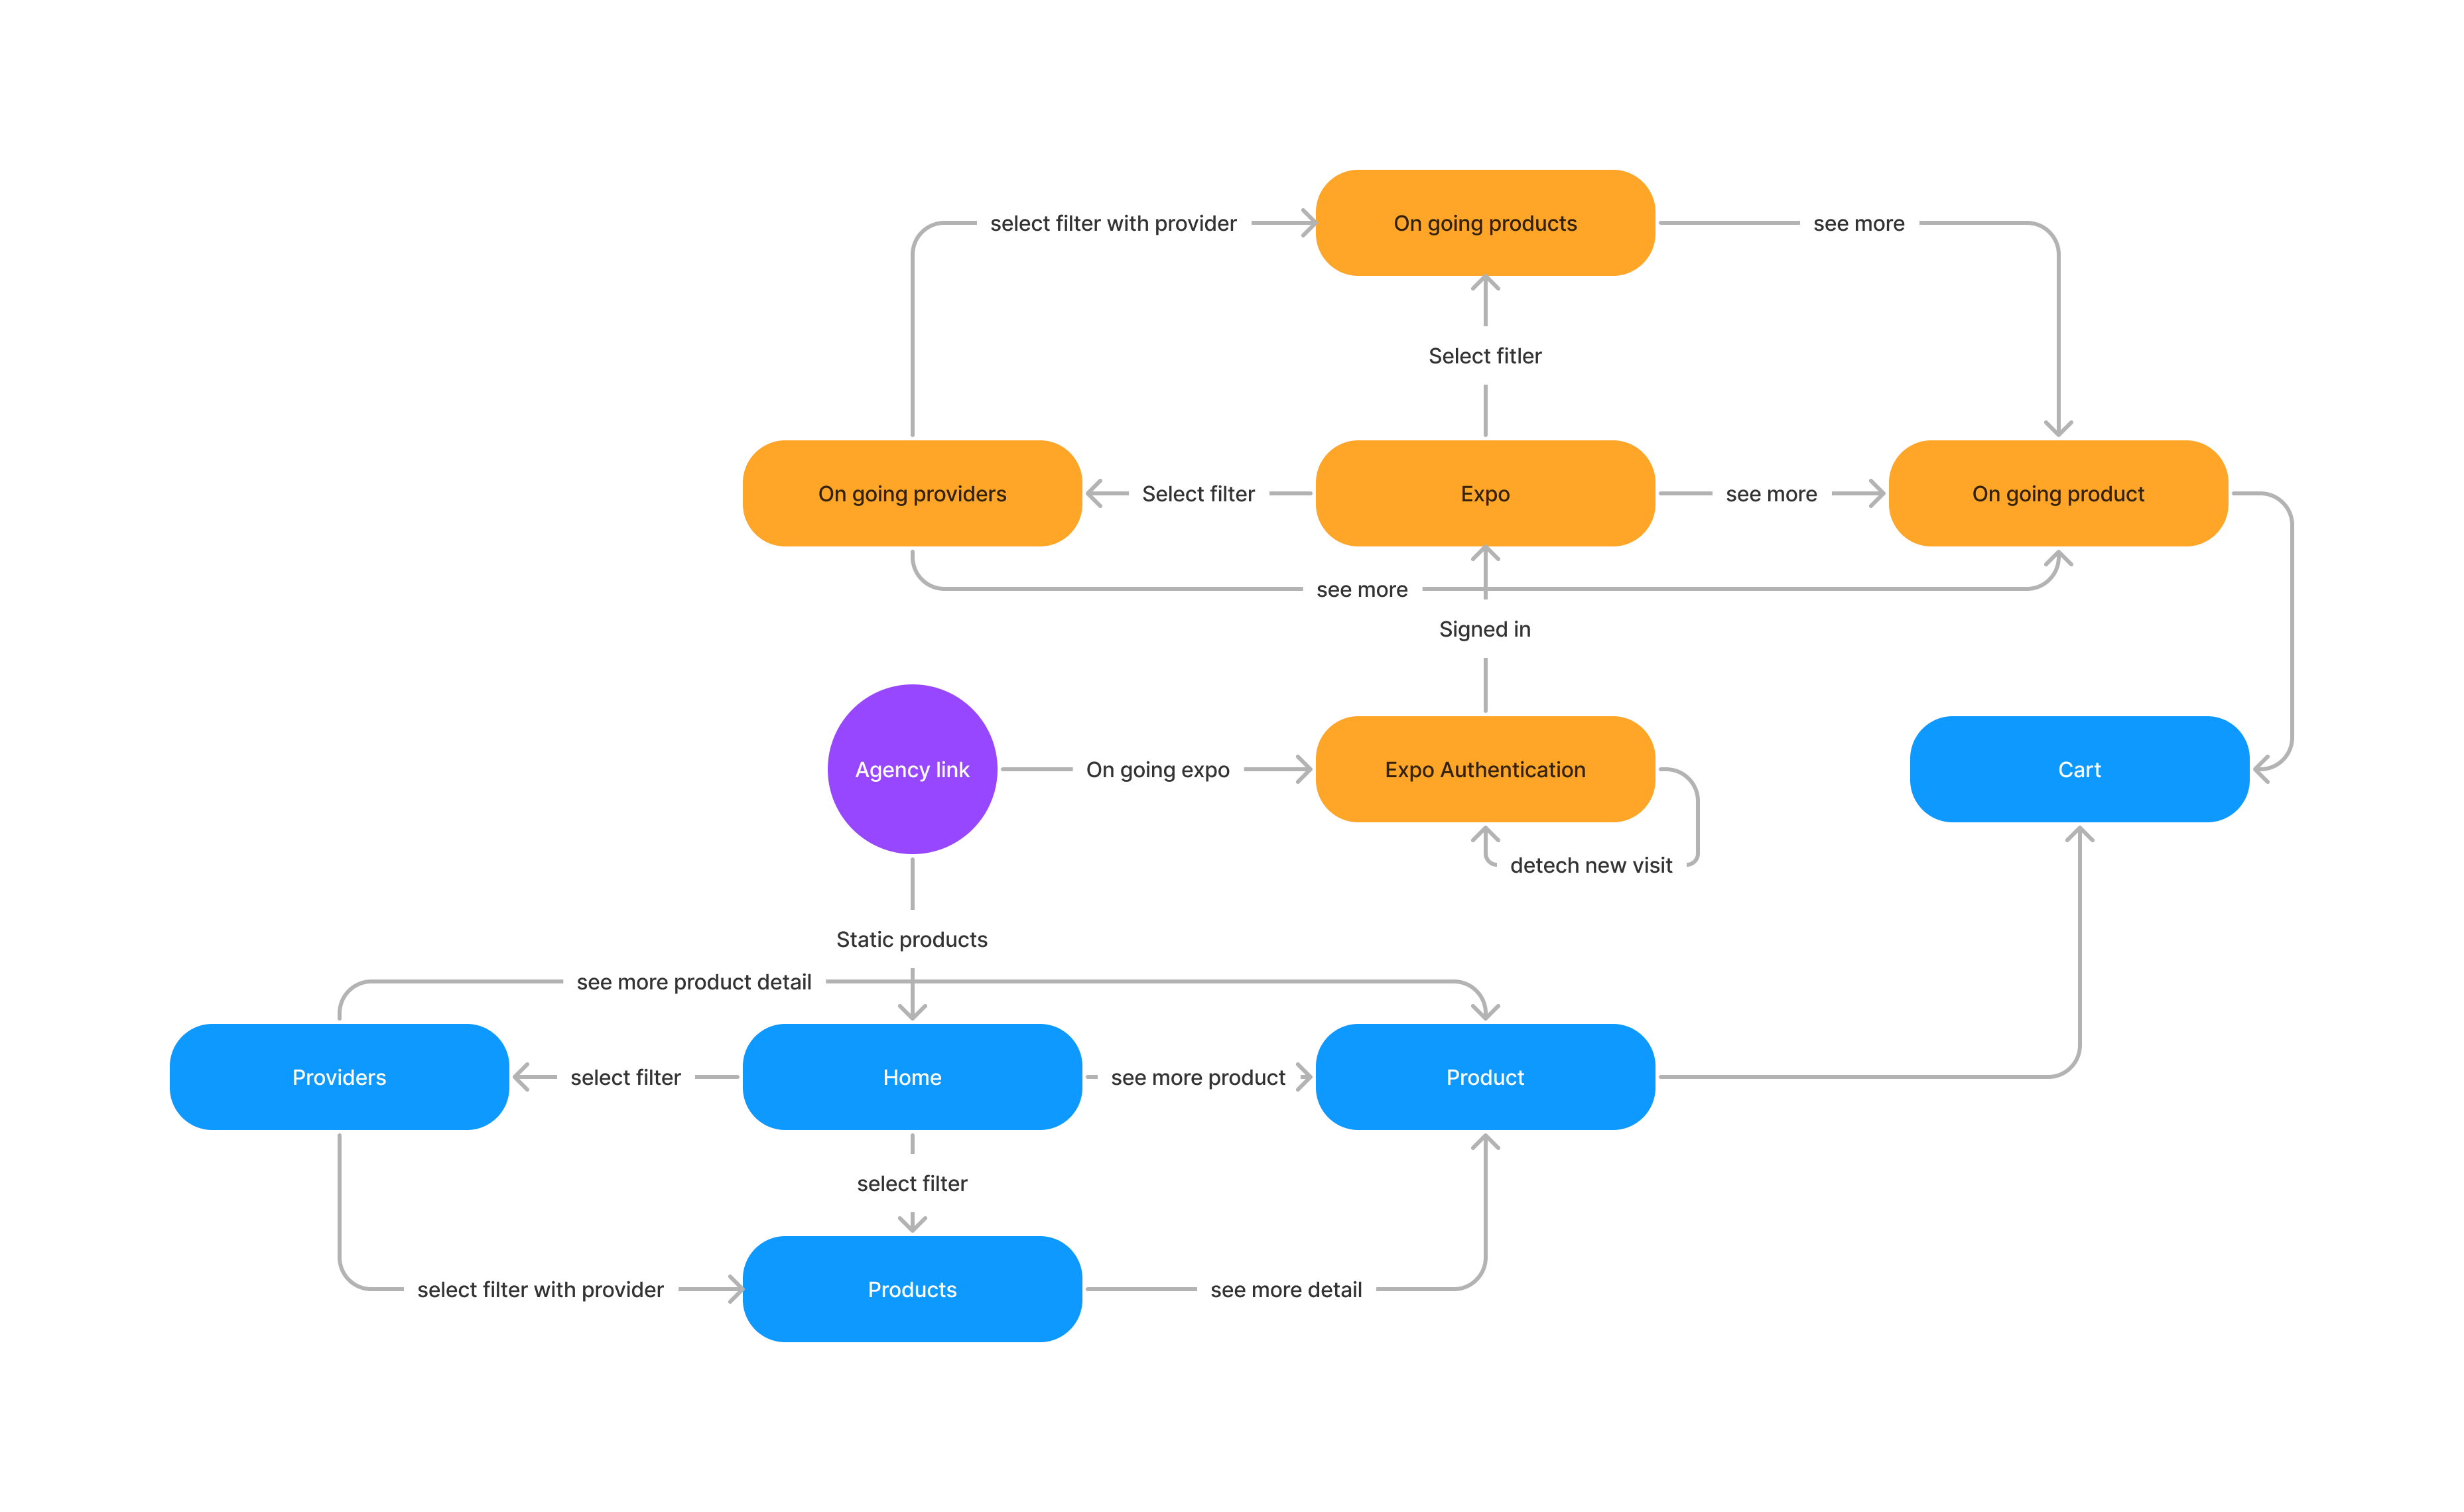
\includegraphics[width=\textwidth]{./images/state.png}
	\label{fig:state}
\end{figure}
As you can see in the figure \ref{fig:state}, the function grows near 0. Also, in the page \pageref{fig:state} is the same example.\pageref{fig:state}


\part{Triển khai và đánh giá}
\chapter{Triển khai}
\section{Requirement}
\subsection{Fundamental}
\begin{itemize}
	\item Hypertext Markup Languageand Cascading Style Sheets.
	\item Javascript, HTML DOM.
  	\item React.js: Virtual DOM, component, element, state, hook.
	\item Unified Modeling Language.
	\item Clients and servers architecture.
	\item Hypertext Transfer Protocol.
\end{itemize}

\subsection{High Level Framework}
\begin{itemize}
\item Chakra UI: Components and Theme.
\item Apollo Client: Queries, Mutations.
\item Itoa JS: Tutorials, GraphQL API Introduction, GraphQL API playground.
\item Next JS: Pages, getServerSideProps, Image Component, Dynamic Routes
\end{itemize}

\section{Guide}
\section{Sources}
https://github.com/ocopee

\subsection{Github ocopee respository}
https://github.com/ocopee/ocopee
\subsection{Github gateway respository}
https://github.com/ocopee/gateway
\subsection{Github accounts respository}
https://github.com/ocopee/accounts
\subsection{Github docs respository}
https://github.com/ocopee/docs
\subsection{Github sellers respository}
https://github.com/ocopee/sellers
\subsection{Installing and setting}
\begin{itemize}
	\item Git
	\item Node.JS (12 or later)
	\item MongoDB (4.4)
\end{itemize}
\subsection{Run server locally}
\subsubsection{Backend}
1. Clone Gateway
\begin{lstlisting}
	git clone gateway_remote_url
\end{lstlisting}
2. Clone submodule
\begin{lstlisting}
	git submodule update --init
\end{lstlisting}
3. Install packages
\begin{lstlisting}
	npm install
\end{lstlisting}
4. Run services and gateway process
\begin{lstlisting}
	# terminal one for accounts service
	npm run dev:accounts
	# terminal two for sellers services
	npm run dev: sellers
	# terminal three for gateway service
	npm run dev
\end{lstlisting}
\subsubsection{Frontend}
1. Clone Gateway
\begin{lstlisting}
	git clone frontend_remote_url
\end{lstlisting}
2. Install packages
\begin{lstlisting}
	npm install
\end{lstlisting}
3. Run client app
\begin{lstlisting}
	npm run dev
\end{lstlisting}
\subsection{Deployment (linux only)}
1. Build project
\begin{lstlisting}
	bash build.sh
\end{lstlisting}
2. Push to remote
\begin{lstlisting}
	git add .
	git commit -m 'commit description'
	git push origin main
\end{lstlisting}
3. Deploy to staging
\begin{lstlisting}
	git checkout staging
	git merge main
	git push origin staging
\end{lstlisting}
4. Deploy to production
\begin{lstlisting}
	git checkout production
	git merge main
	git push origin production
\end{lstlisting}
\section{History}

\subsection{Client App CI (Front-end)}
\begin{figure}
	\centering
	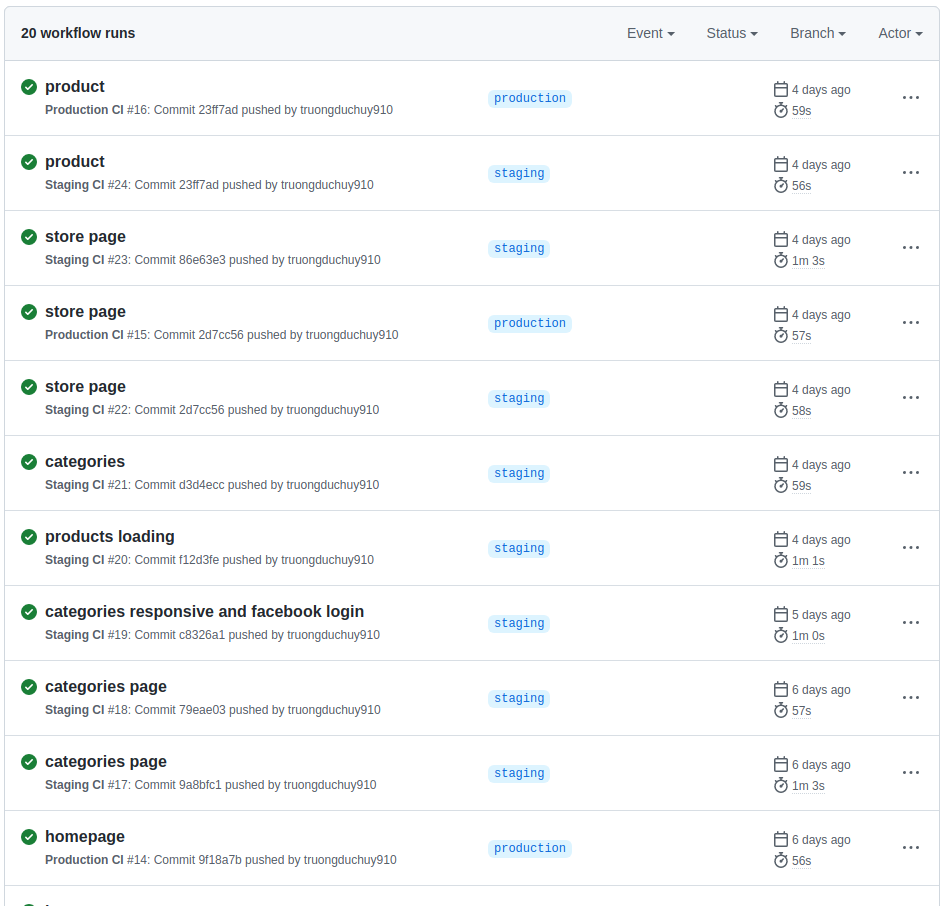
\includegraphics[width=1\linewidth]{./images/ocope-actions}
	\caption[Client app actions]{Client app actions}
	\label{fig:ocope-actions}
\end{figure}


\subsection{Gateway App CI (Back-end)}

\begin{figure}
	\centering
	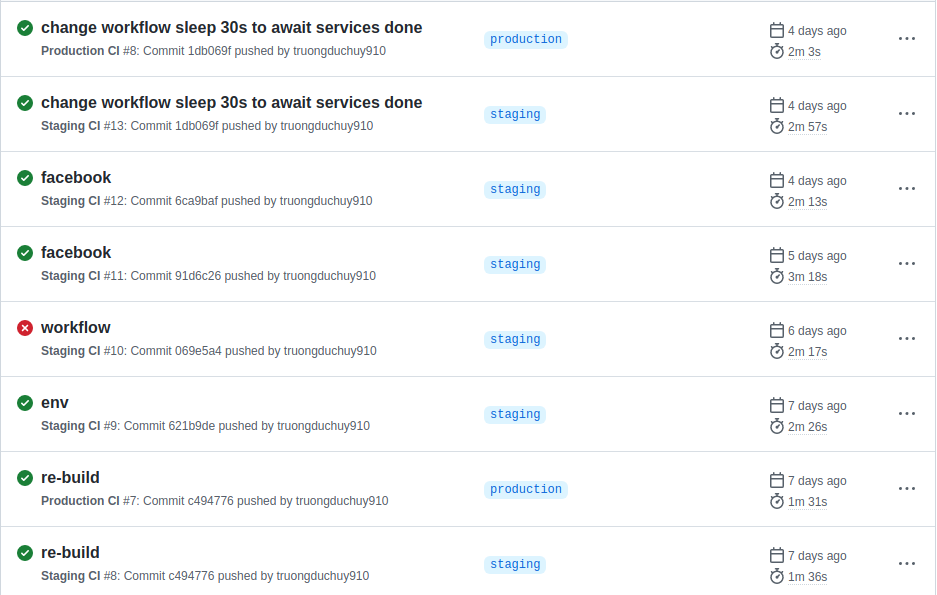
\includegraphics[width=1\linewidth]{./images/gateway-actions}
	\caption[Gateway actions]{Gateway actions history.}
	\label{fig:gateway-actions}
\end{figure}


\section{Position}
\chapter{Đánh giá}
1. Developer

1.1 Leader

Abbreviation is DL

Missions:

- Feedback task
- Deploy task
- Merge task
- Approval task
- Review task
- Complex task
- Investigate

1.2. Backend

Abbreviation is BE

Missions:

- Server-side task
- Reviewing task
- Client-side logic task

Workings:

1.2 Frontend

Abbreviation is FE

Missions:

- Client-side task
- Client-side logic task
- Reviewing task
- UX/UI task

1.3 Manager

Abbreviation is MN 

Missions:

- Ideas
- Planing

\part*{Kết luận và hướng phát triển}

\chapter{Kết quả đạt được}
\chapter{Những vấn đề hạn chế}
\chapter{Hướng phát triển}
 Phân quyền

Quyền sở hữu (owner)

Ai tạo thì người đó mới có quyền xóa.

> THAY ĐỔI QUAN TRỌNG: Tất cả các bảng đều phải có byTracking. Bởi vì, mối liên hệ giữa các bảng có thể thay đổi nhưng
> quyền sở hữu giữa dữ liệu đó và người sở hữu không thay đổi.

> Nếu tạo ra dữ liệu mà không đăng nhập, thì dữ liệu sẽ thuộc về người sở hữu domain trong headers của request hiện tại.
> [chi tiết](quyền-tạo) xem bên dưới.

> Khi tạo đơn đặt hàng, tạo nội dung, dữ liệu sản phẩm cho người khác. Phải quyển quyền sở hữu sau đó. Và ghi thông tin
> người tạo vào dữ liệu nếu cần. Nhưng bản chất dữ liệu đó đã chuyển quyền sở hữu rồi.

Chuyển quyền sở hữu:

Coi như người được chuyển tạo ra dữ liệu đó. nghĩa là, sau khi chuyển người sở hữu cũ không có quyền xóa nữa.

> Tóm lại, A sở hữu thì createdBy: { id: A.id }

Quyền xem (read)

Quyền xem đa dạng hơn tùy trường hợp sử dụng.

-   Quyền xem mặc định, quyền xem cụ thể cho bảng dữ liệu, trường dữ liệu. Quyền xem cụ thể sẽ ghi đè quyền xem tổng hơn
hơn nó chứ không kế thừa.

-   Chia ra làm hai loại là phân quyền trực tiếp và phân quyền gián tiếp.

-   Phân quyền cho loại dữ liệu và phân quyền cho dữ liệu (bản ghi) cụ thể.

Chi tiết:

-   Đối với phân quyền trực tiếp thì người tạo ra, người sở hữu dữ liệu toàn quyền xem với dữ liệu đó.
-   Phân quyền gián tiếp cho "loại dữ liệu" phải thông qua bảng phân quyền. Bản phân quyền này tạo bởi người sở hữu dữ
liệu. Nghĩa là tôi cấp quyền cho một người cụ thể xem toàn bộ dữ liệu thuộc bảng A.
-   Ngoài ra, một số kiểu dữ liệu phục vụ cho việc quảng cáo và truyền thông, thì có thể thông qua domain mà không cần
đăng nhập. Nghĩa là khi truy cập dữ liệu thông qua domain, một người bất kì có thể xem dữ liệu được tạo ra bởi người
sử hữu domain. Chi tiết tại phân quyền của seller.
> domain có thể được ghi đè để sử dụng trong một số trường hợp như dùng chung admin ui, dùng mobile app.
-   Phân quyền gián tiếp cho "dữ liệu" (bản ghi) cụ thể cần ghi cụ thể id người được phân quyền trong tập dữ liệu. Tên
của trường đó đặt tùy trường hợp sử dụng.
-   Phân quyền gián tiếp cho "dữ liệu" (bản ghi) cụ thể cho nhiều người xem chưa được xem xét phát triển. Nhưng có thể
tạo bảng phần quyền cụ thể riêng. Bảng này người sở hữu chỉ định bản ghi cụ thể này được chia sẽ cho ai.

> Xem sản phẩm được tạo ra bởi tôi (read) A là người sở hữu dữ liệu thì createdBy: { id: A.id }


> LƯU Ý QUAN TRỌNG: Người dùng chấp nhận lời mời vào nhóm. Được cấp quyền xem một số bảng của tổ chức nhưng cũng đồng
> thời chia sẽ quyền xem toàn bộ dữ liệu của mình cho tổ chức đó ngoại trừ mật khẩu.

Xem sản phẩm được tạo ra cho tôi bởi người không xác định, hoặc thành viên của tổ chức (read-of)



> Với thay đổi gần nhất, thì id của of này cần ghi đề vào createdBy bằng cách bấm chấp nhận sở hữu, hoặc cài tự động
> chấm nhận.

Xem sản phẩm được chia sẽ với tôi (read-by)

Như đã đề cập ở phân quyền gián tiếp. Ta định hướng chia sẻ toàn bộ dữ liệu thuộc bảng A và chia sẻ bản ghi cụ thể:

Đối với chia sẽ toàn bộ bảng A:

-   Dữ liệu được chia sẽ thông qua nhóm thuộc tổ chức. Một người sở hữu một tổ chức. Tổ chức sở hữu nhiều nhóm. Các nhóm
sẽ được phân quyền đọc hoặc chỉnh sửa các bảng cụ thể.

Đối với chia sẽ bản ghi cụ thể:

-   Chưa phát triển.

Quyền tạo

Yều cầu đăng nhập

1. Tạo cho chính họ: byTracking sẽ điền thông tin là người đăng nhập hiện tại.
2. Tạo cho người khác: Cũng là tạo cho chính họ, nhưng of đặt id người cần chuyển quyền sở hữu. Khi người được chuyển
bấm xác nhận, hoặc tự động xác nhận thì ghi đè quyền sở hữu và xóa trường of đi.

Không yêu cầu đăng nhập

1. Không yêu cầu đăng nhập thì mặc định là tạo hộ cho người sở hữu domain.

> Lập trình viên cần lưu ý chỗ tạo và liên kết các dữ liệu. Khi người tạo liên kết dữ liệu họ không sở hữu.

> Cần lưu ý `of` khi không đăng nhập là tự điền, còn khi có đăng nhập là có thể chọn hoặc tự điền nếu người tạo bỏ
> trống.

Quyền chỉnh sửa

Ai tạo thì người đó có quyền sửa và có thể sửa hộ.

-   byTracking lúc này là `createdBy: null` nên vẫn đặt of là id người được chuyển như bình thường. Người nhận dữ liệu
bấm xác nhận hoặc tự động xác nhận ghi thông tin id từ of vào createdBy.

Chỉnh sửa sản phẩm của tôi (update)

Chỉnh sửa sản phẩm tạo ra cho tôi bởi người không xác định



 Phân quyền

Quyền sở hữu (owner)

Ai tạo thì người đó mới có quyền xóa.

> THAY ĐỔI QUAN TRỌNG: Tất cả các bảng đều phải có byTracking. Bởi vì, mối liên hệ giữa các bảng có thể thay đổi nhưng quyền sở hữu giữa dữ liệu đó và người sở hữu không thay đổi.

> Nếu tạo ra dữ liệu mà không đăng nhập, thì dữ liệu sẽ thuộc về người sở hữu domain trong headers của request hiện tại. [chi tiết](quyền-tạo) xem bên dưới.

> Khi tạo đơn đặt hàng, tạo nội dung, dữ liệu sản phẩm cho người khác. Phải quyển quyền sở hữu sau đó. Và ghi thông tin người tạo vào dữ liệu nếu cần. Nhưng bản chất dữ liệu đó đã chuyển quyền sở hữu rồi.

Chuyển quyền sở hữu:

Coi như người được chuyển tạo ra dữ liệu đó.
nghĩa là, sau khi chuyển người sở hữu cũ không có quyền xóa nữa.

> Tóm lại, A sở hữu thì createdBy: { id: A.id }

Quyền xem (read)

Quyền xem đa dạng hơn tùy trường hợp sử dụng.

- Quyền xem mặc định, quyền xem cụ thể cho bảng dữ liệu, trường dữ liệu. Quyền xem cụ thể sẽ ghi đè quyền xem tổng hơn hơn nó chứ không kế thừa.

- Chia ra làm hai loại là phân quyền trực tiếp và phân quyền gián tiếp.

- Phân quyền cho loại dữ liệu và phân quyền cho dữ liệu (bản ghi) cụ thể.

Chi tiết:

- Đối với phân quyền trực tiếp thì người tạo ra, người sở hữu dữ liệu toàn quyền xem với dữ liệu đó.
- Phân quyền gián tiếp cho "loại dữ liệu" phải thông qua bảng phân quyền. Bản phân quyền này tạo bởi người sở hữu dữ liệu. Nghĩa là tôi cấp quyền cho một người cụ thể xem toàn bộ dữ liệu thuộc bảng A.
- Phân quyền gián tiếp cho "dữ liệu" (bản ghi) cụ thể cần ghi cụ thể id người được phân quyền trong tập dữ liệu. Tên của trường đó đặt tùy trường hợp sử dụng.
- Phân quyền gián tiếp cho "dữ liệu" (bản ghi) cụ thể cho nhiều người xem chưa được xem xét phát triển. Nhưng có thể tạo bảng phần quyền cụ thể riêng. Bảng này người sở hữu chỉ định bản ghi cụ thể này được chia sẽ cho ai.

> Xem sản phẩm được tạo ra bởi tôi (read) A là người sở hữu dữ liệu thì createdBy: { id: A.id }

Xem sản phẩm được tạo ra cho tôi bởi người không xác định, hoặc thành viên của tổ chức (read-of)


> Với thay đổi gần nhất, thì id của of này cần ghi đề vào createdBy bằng cách bấm chấp nhận sở hữu, hoặc cài tự động chấm nhận.

Xem sản phẩm được chia sẽ với tôi (read-by)

Như đã đề cập ở phân quyền gián tiếp. Ta định hướng chia sẻ toàn bộ dữ liệu thuộc bảng A và chia sẻ bản ghi cụ thể:

Đối với chia sẽ toàn bộ bảng A:

- Dữ liệu được chia sẽ thông qua nhóm thuộc tổ chức.
Một người sở hữu một tổ chức. Tổ chức sở hữu nhiều nhóm.
Các nhóm sẽ được phân quyền đọc hoặc chỉnh sửa các bảng cụ thể.

Đối với chia sẽ bản ghi cụ thể:

- Chưa phát triển.

Quyền tạo

Yều cầu đăng nhập

1. Tạo cho chính họ:
byTracking sẽ điền thông tin là người đăng nhập hiện tại.
2. Tạo cho người khác:
Cũng là tạo cho chính họ, nhưng of đặt id người cần chuyển quyền sở hữu. Khi người được chuyển bấm xác nhận, hoặc tự động xác nhận thì ghi đè quyền sở hữu và xóa trường of đi.

Không yêu cầu đăng nhập

1. Tạo cho người khác
> Lập trình viên cần lưu ý chỗ tạo và liên kết các dữ liệu. Khi người tạo liên kết dữ liệu họ không sở hữu.

Quyền chỉnh sửa

Ai tạo thì người đó có quyền sửa và có thể sửa hộ.

- byTracking lúc này là `createdBy: null` nên vẫn đặt of là id người được chuyển như bình thường. Người nhận dữ liệu bấm xác nhận hoặc tự động xác nhận ghi thông tin id từ of vào createdBy.

Chỉnh sửa sản phẩm của tôi (update)

Chỉnh sửa sản phẩm tạo ra cho tôi bởi người không xác định



Addmission

Yêu cầu tham gia nhóm từ tổ chức gửi cho một cá nhân cụ thể. Chỉ người sở hữu tổ chức (chứa nhóm này) và người được gửi
lời mời được quyền xem.

Sau khi chấp nhận lời mời, người sở hữu tổ chức có thể xem và sử dụng dữ liệu của thành viên cho mục đích phân phối,
trình bày, quảng cáo.

Nếu người được mời hủy chấp nhận thì các quyền nêu trên mất hiệu lực.


Issue
Vấn đề, công việc của nhóm.

Người sở hữu tổ chức. Người tham gia nhóm có quyền xem thông tin này.

IssueType
Phân quyền giống như Issue



 Định nghĩa các môi trường khi chạy phần mềm.

1. Môi trường phát triển cục bộ (development)

Tất cả các tiến trình, máy chủ cơ sở dữ liệu đề chạy cục bộ.

2. Môi trường phát triển nhanh (testing)

Một số tiến trình, máy chủ cơ sở dữ liệu được cài đặt khởi chạy trên máy chủ kiểm thử.

Kết nối với cơ sở dữ liệu kiểm thử.

3. Môi trường tiền phát hành (staging)

Tất cả tiến trình và máy chủ cơ sở dữ liệu được cài đặt khởi chạy trên máy chủ kiểm thử.

Kết nối với cơ sở dữ liệu phát hành.

4. Môi trường phát hành. (production)

Tất cả tiến trình được cài đặt và khởi chạy trên máy chủ phát hành.

Kết nối với cơ sở dữ liệu kiểm thử phát hành.



Với mục đích làm cửa ngõ cho client projects như: next.js server, mobile app.

Gateway server không thực hiện chức năng mà gom các chức năng lại tại một end-point duy nhất.

Gateway đồng thời cũng phát triển một admin ui chung cho tất cả các services.

> Điều quan trọng cần nhớ là hạn chế càng nhiều vai trò của gateway trong hệ thống càng tốt.



 Nhu cầu quản lí lao động thời vụ

Các trường hợp sử dụng

-   Đăng tuyển và quản lí thông tin người ứng tuyển.
-   Nhắc nhở người tuyển dụng và người ứng tuyển về lịch hẹn.
-   Tạo, xác nhận, kết thúc các loại hợp đồng.
-   Báo cáo các công việc hoàn thành trong ngày.
-   Xác nhận báo cáo công việc.
-   Chấm công theo "đơn vị công việc" hoàn thành.
-   Tính lương theo đơn vị công việc hoàn thành và khung lương của loại công việc đó. Cụ thể theo thời gian thì công
việc là dọn dẹp, trực ca, bán hàng, gia công sơ chế,... Theo khối lượng thì theo sản phẩm làm ra, gia công được,...
-   Đánh giá năng lực sau khi phỏng vấn, năng suất theo từng loại "đơn vị công việc".
-   Quản lí ứng lương.
-   Duyệt yêu cầu ứng lương.
-   Quản lí yêu cầu chốt lương hoặc tự động chốt lương vào ngay cụ thể.
-   Xác nhận chuyển lương đã chốt.

Ví dụ 1

Nhân viên Tèo được phỏng vấn vào làm các công việc: Gia công, trực cửa hàng, đóng gói, giao hàng.

Tèo làm buổi sáng 4 tiếng gia công. Buổi chiều trực cửa hàng 3 tiếng. Đóng gói 1 tiếng. Làm xong tèo báo cáo vào bảng
rồi đi về.

Tí buổi hôm sau chấm công cho Tèo 4 tiếng gia công được 80.000đ. 3 tiếng trực ca được 45.000đ và 1 tiếng đóng gói được
22.000đ. Tổng cộng 147.000đ

Rồi Tèo lại tiếp tục làm công việc gia công, nhưng hôm nay sản phẩm Tèo làm quen tay, Tèo muốn làm và báo cáo theo sản
phẩm. Tèo làm được 10 sản phẩm trong 4 tiếng. Buổi chiều Tèo đi giao hàng. Xong việc Tèo báo cáo nhận lương và đi về.

Rồi ngày hôm sau đáng lẽ hôm nay Tèo được nhận 100.000đ gia công tính theo sản phẩm. Và 4 tiếng đi giao hàng được
120.000đ. Tổng cộng 220.000đ. Nhưng Tí bị ốm và không trả công được cho Tèo. Nên Tèo hôm đó phải nghỉ nhậu.

Tháng sau Tèo quyết định không nhậu nữa và muốn nhận lương một lần vào cuối tháng. Tèo cũng rất quyết tâm kiếm tiền nên
quyết định tăng ca. Công việc khi tăng ca giống với công việc bình thường nhưng lương cao hơn. Tèo cũng hay mở điện
thoại ra để kiểm tra xem mình đã tích góp được bao nhiêu tiền.

Tí cảm thấy Tèo rất nhiệt tình nên đã quyết định thưởng thêm cho Tèo một số tiền vào một số buổi tăng ca.

Nhưng trước ngày chốt lương 3 ngày. Tèo lại muốn mua một con robot. Nên Tèo quyết định chốt lương sớm và ứng trước một
số tiền.

Tí thấy yêu cầu của Tèo là hợp lí và sẽ chuyển tiền trong vòng 3 ngày cho Tèo.

Phân tích vai trò

[Sơ đồ ](https://www.figma.com/file/RDcs6EJcCUofJYmV3GUOPi/Ch%E1%BA%A5m-c%C3%B4ng?node-id=0%3A1)


\bibliographystyle{alpha}
\bibliography{website}

\end{document}